\chapter{\label{method}Experimental Set-up}
Two metal rulers are fixed vertically at the bottom and are capable of vibrating with small amplitudes, acting as oscillators that are coupled by a rubber band, similar to a two-mass and three-spring system. The mass and elastic moduli of the rulers correspond to the mass and spring constant of an oscillator, with the first ruler behaving like a mass attached to a rigid wall with a spring constant in Figure 1, while the second ruler behaves like another mass with its own spring constant. The rubber band connecting the two rulers acts as a coupling spring. Assuming small amplitudes, the vibration of the rulers, including the angular displacement of any segment from the vertical, can be modelled as simple harmonic motion. 

The displacements of the rulers are accurately measured using a He-Ne laser beam. The beam is split into two polarized beams using a polarizing cube beam splitter (PBS1), and the transmitted beam passes through a quarter-wave plate to make it circularly polarized. The beam is then reflected by a mirror attached to the ruler and passes through the quarter-wave plate again, making it linearly polarized with a phase shift of $\pi$/2 relative to the transmitted beam. The reflected beam is then reflected by PBS1 onto the quad photodetector D1 instead of being transmitted back to the laser source. The polarized beam reflected by PBS1 is then reflected by a second polarizing beam splitter (PBS2) and is again passed through the quarter-wave plate before being reflected by the plane mirror attached to the ruler. When the ruler undergoes small oscillations, the reflected beam makes an angular displacement along the normal line. The larger the displacement of the ruler, the greater the angular displacement of the reflected beam. The reflected beam falls onto the quad photodetector, and the signals detected by the upper and lower halves of the detector are separately amplified with the same gain and then subtracted. As the laser spot moves upward from the mean position, the upper two photo-detectors detect a larger signal than the lower two photo-detectors, and vice versa when the laser beam moves downward. Consequently, the difference between the output voltages of the two halves oscillates proportionally to the displacement of the oscillating ruler. This difference is then normalized to make an analogy with Rabi oscillation. The schematic setup is shown in Figure. (3)\footnote{Sharba Bhattacharjee et al 2018 Eur. J. Phys. 39 035404}.
\begin{figure}[H]
	\centering
	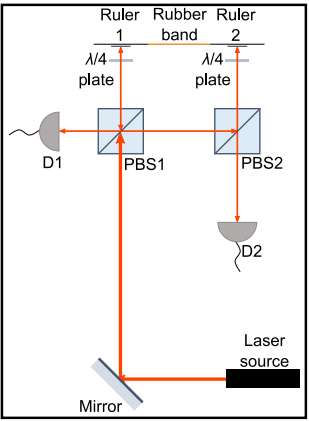
\includegraphics[scale=0.8]{setup diagram.png}
	\caption{ Schematic diagram of the
		experimental set-up (top view) showing the path taken by the laser beam. PBS1, PBS2:polarising cube beam splitters; D1, D2: quad photodetectors}
	\label{fig:mb-fe-0}
\end{figure}
\begin{figure}[H]
	\centering
	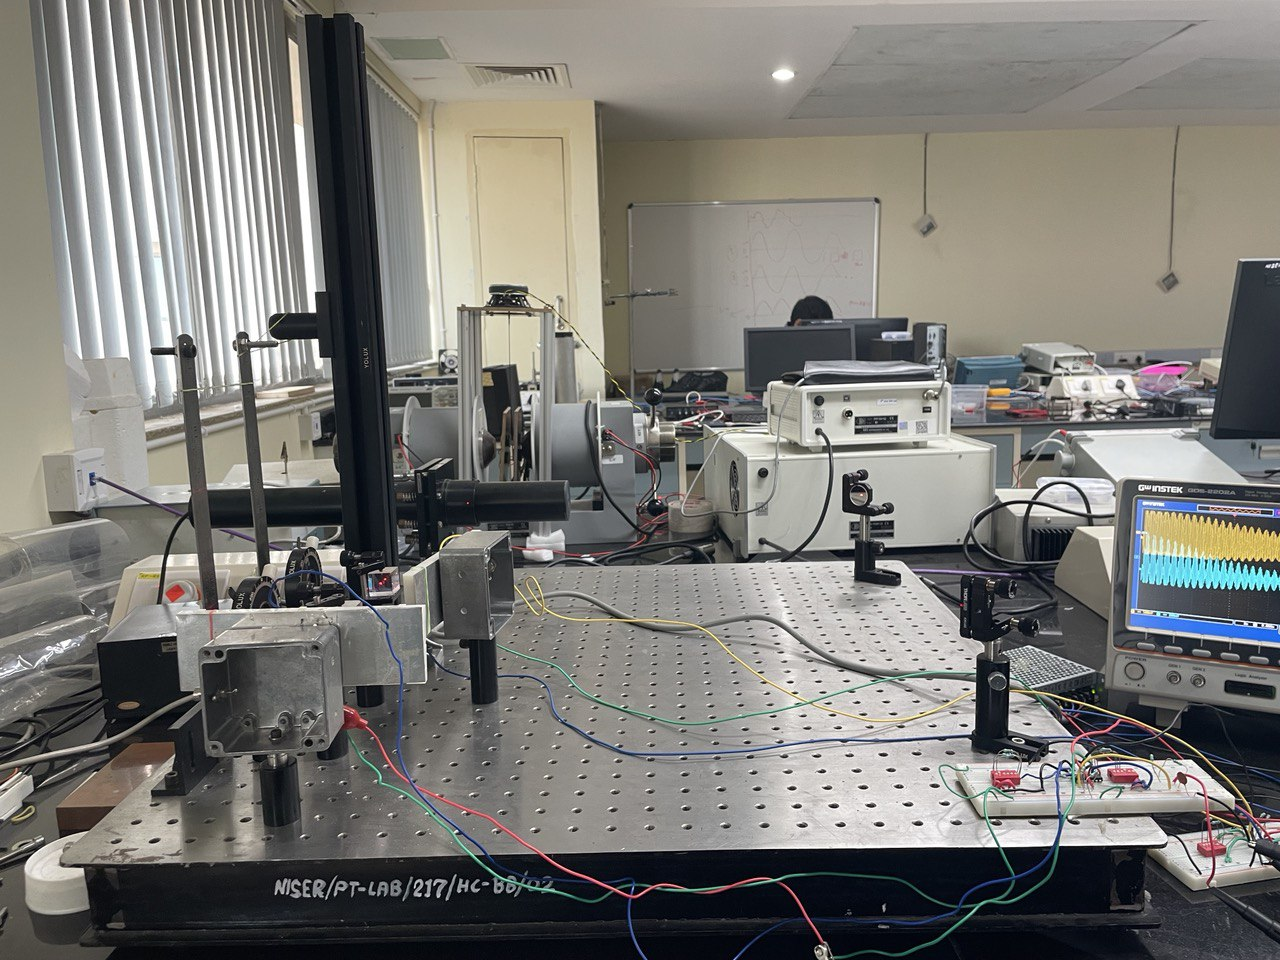
\includegraphics[scale=0.3]{setup.jpeg}
	\caption{Overview of our experimental set-up. Notice the the black pillar we set-up for our innovation part. That beam was mounted and a rubber band was tied to this beam and one of the rulers. This extra rubber band induced the dampening.}
	\label{fig:mb-fe-0}
\end{figure}
The quad photo-detector comprises four photo-diodes arranged in a square cell, with the upper two detecting the upper signal of the moving laser spot and the lower two detecting the lower signal. To amplify the signals, we utilized the TL084 op-amp due to its superior slew rate and high-frequency response. The amplified signals are then subtracted using a differential amplifier (also TL084) to yield a signal voltage proportional to the displacement of the ruler. To eliminate high-frequency noise in our circuit, we incorporated an RC low pass filter. The signal is ultimately viewed through an oscilloscope, with the cut-off frequency of the RC filter set at 88.42Hz.
\begin{figure}[H]
	\centering
	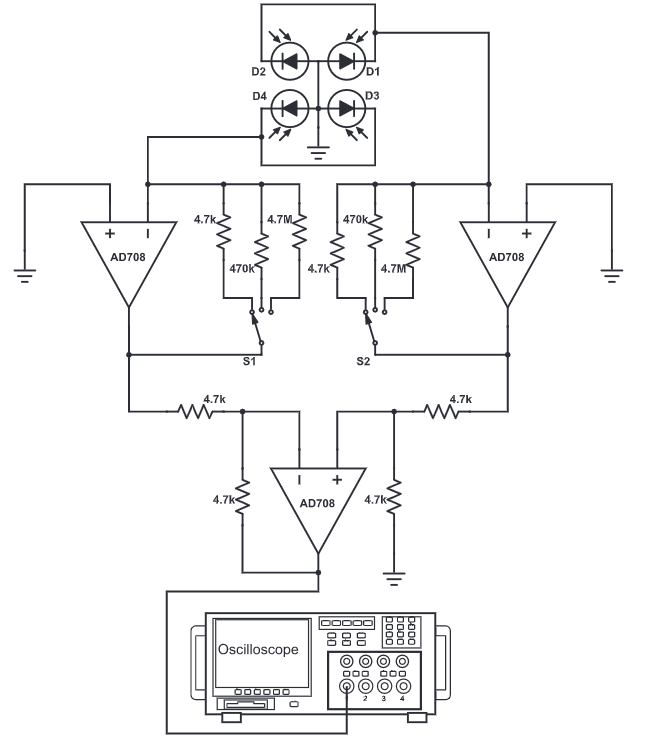
\includegraphics[scale=0.7]{screenshot001}
	\caption{This is the TL084/AD708 circut diagram that was used to relay the voltage detcted by the photodetector.}
	\label{fig:screenshot001}
\end{figure}
\begin{figure}[H]
	\centering
	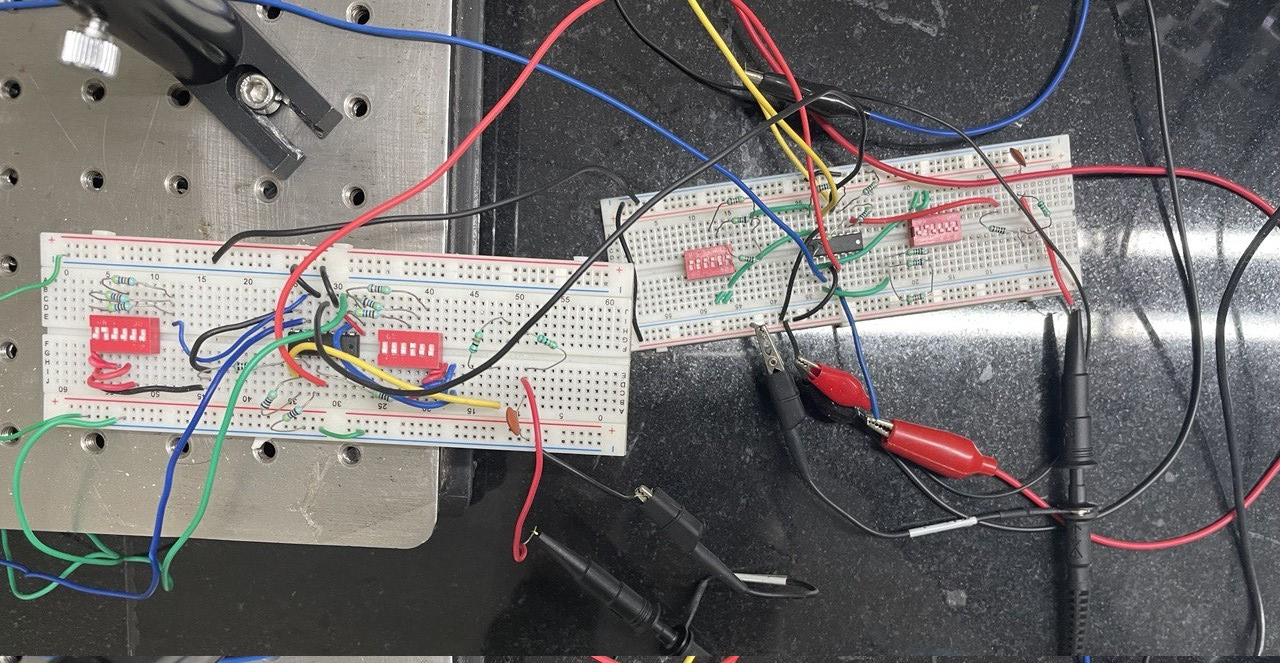
\includegraphics[scale=0.3]{breadboard.jpeg}
	\caption{The circuitry of the amplifier (TL084) that was used to relay the data into our oscilloscope}
	\label{fig:mb-fe-0}
\end{figure}


%\baselineskip 24pt
